\chapter{Desenvolvemento do sistema}
\minitoc
\label{chap:implementacion}
\vspace{0.5cm}

%%%%%%%%%%%%%%%%%%%%%%%%%%%%%%%%%%%%%%%%%%%%%%%%%%%%%%%%%%%%%%%%%%%%%%%%%%%%%%%%
% Objetivo: Exponer las partes relevantes de la implementación                 %
%%%%%%%%%%%%%%%%%%%%%%%%%%%%%%%%%%%%%%%%%%%%%%%%%%%%%%%%%%%%%%%%%%%%%%%%%%%%%%%%

\lettrine{N}{este} capítulo exporase o desenvolvemento do proxecto baseándose
no esquema proporcionado pola planificación inicial: desde o deseño software e
hardware de baixo nivel do sistema ata a implementación e o ensamblado do
producto, pasando por un prototipo operacional.

\section{Determinación}

 \subsection{Obxectivos}

 Establecéronse os obxectivos da fase de desenvolvemento do proxecto. \\

 Obxectivos:

 \begin{itemize}
  \item Implementar unha gaita MIDI sen fíos en tempo real empregando
        software/hardware libre.
 \end{itemize}

 \subsection{Alternativas}

 Establecéronse posibles alternativas a eses obxectivos, aplicables no caso de
 que estes non se puidesen cumprir. \\

 Alternativas:

 \begin{itemize}
  \item Se non é posible implementar completamente o proxecto, pode optarse
        por:
        \begin{enumerate}
         \item Se é por causa de que o hardware non o permite, cambiar as pezas
               correspondentes por outras que si o permitan.
         \item Se as partes que non é posible implementar son opcionais ou de
               pouco peso, desbotalas e implementar o resto.
         \item Cancelar e mudar de proxecto.
        \end{enumerate}
 \end{itemize}

 \subsection{Restriccións}

 Establecéronse restriccións aplicables a ditos obxectivos.

 \begin{enumerate}
  \item As propias restriccións veñen dadas polo propio título do proxecto. A
        saber:
        \begin{enumerate}
         \item Empregar o protocolo MIDI.
         \item Empregar tecnoloxía sen fíos.
         \item Empregar tempo real.
         \item Empregar software libre.
         \item Empregar harwdware libre.
         \item E/ou as derivadas de calquera das súas alternativas.
        \end{enumerate}
 \end{enumerate}

\section{Avaliación de alternativas e resolución de riscos}

 \subsection{Análise de riscos}

 Determináronse os riscos que comportaban as distintas alternativas e as súas
 posibles solucións.

 \begin{enumerate}
  \item Alternativas 1.
        \begin{enumerate}
         \item Riscos:
               \begin{enumerate}
                \item Que non exista hardware alternativo que soporte a
                      implemtación das características restantes.
                \item Que as partes a desbotar sexan partes importantes ou
                      incluso críticas.
                \item Que o tempo restante para a execución do proxecto non
                      sexa suficiente.
               \end{enumerate}
         \item Solucións:
               \begin{enumerate}
                \item Recortar características ou cancelar e mudar de proxecto.
                \item Aplicar medidas de mitigación para que a planificación
                      non se vexa afectada en extremo, ou cancelar e mudar de
                      proxecto se fan inviable o mesmo.
                \item Agardar a presentalo na seguinte convocatoria.
               \end{enumerate}
        \end{enumerate}
 \end{enumerate}

 \subsection{Prototipo operacional}
 
 Nesta fase desenvolveuse o seguinte nivel de prototipado, tanto hardware coma
 software, sendo xa ambos operacionais. \\
 
 A aproximación seguida foi aplicar \textit{BDD} \cite{BDD} ou \textit{TDD}
 \cite{TDD} segundo o caso, en dirección \textit{top-dowm} obtendo así as
 sinaturas dos servizos e o comportamento desexado dos mesmos primeiro, para
 logo facer unha implementación \textit{bottom-up} respectando o deseño
 conseguido previamente.

  \subsubsection{Prototipo hardware}
  
  Para a o prototipo hardware operacional tiramos do prototipo deseñado na fase
  anterior, para o cal empregamos ferramentas CAD co fin de poder facer probas
  en formato dixital antes de pasar a formato físico, evitando así os múltiples
  problemas relacionados.

   \paragraph{Integración do hardware}
   
   Unha vez claro o deseño sobre o papel, montouse un prototipo físico con cada
   compoñente por separado, de maneira que inicialmente se puidera probar cada
   un de maneira unitaria, antes de pasar á integración final. \\
   
   Desta maneira, dividiuse a montaxe completa en varias submontaxes:
   
   \begin{itemize}
    \item Router (figura \ref{figura:Router}).
    \item Receptor (figura \ref{figura:Receptor}).
    \item Sensor de presión (figura \ref{figura:SensorPresion}).
    \item Sensores capacitivos (figura \ref{figura:SensoresCapacitivos}).
    \item Lector de tarxetas (figura \ref{figura:LectorTarxetas}).
   \end{itemize}
   
   A primeira montaxe foi a do router por resultar a máis sinxela, xa que
   consistiu nunha placa Arduino Uno sobre a que se montou unha placa auxiliar
   onde se montou o transmisor XBee, todo sen maior problema por ser altamente
   acoplables, sendo logo embebidos nunha caixa a medida e conectados por USB
   ó ordenador onde se executa a aplicación de configuración e o servidor
   MIDI. \\
   
   A nivel de sinatura de servizos, ó funcionar coma un simple router
   automatizado, non tiña máis que probar a transmisión correcta de datos, que
   decidiu deixarse coma último punto da integración hardware por razóns de
   escalibidade e fiabilidade. \\
   
   \begin{figure}[htbp]
    \centering
    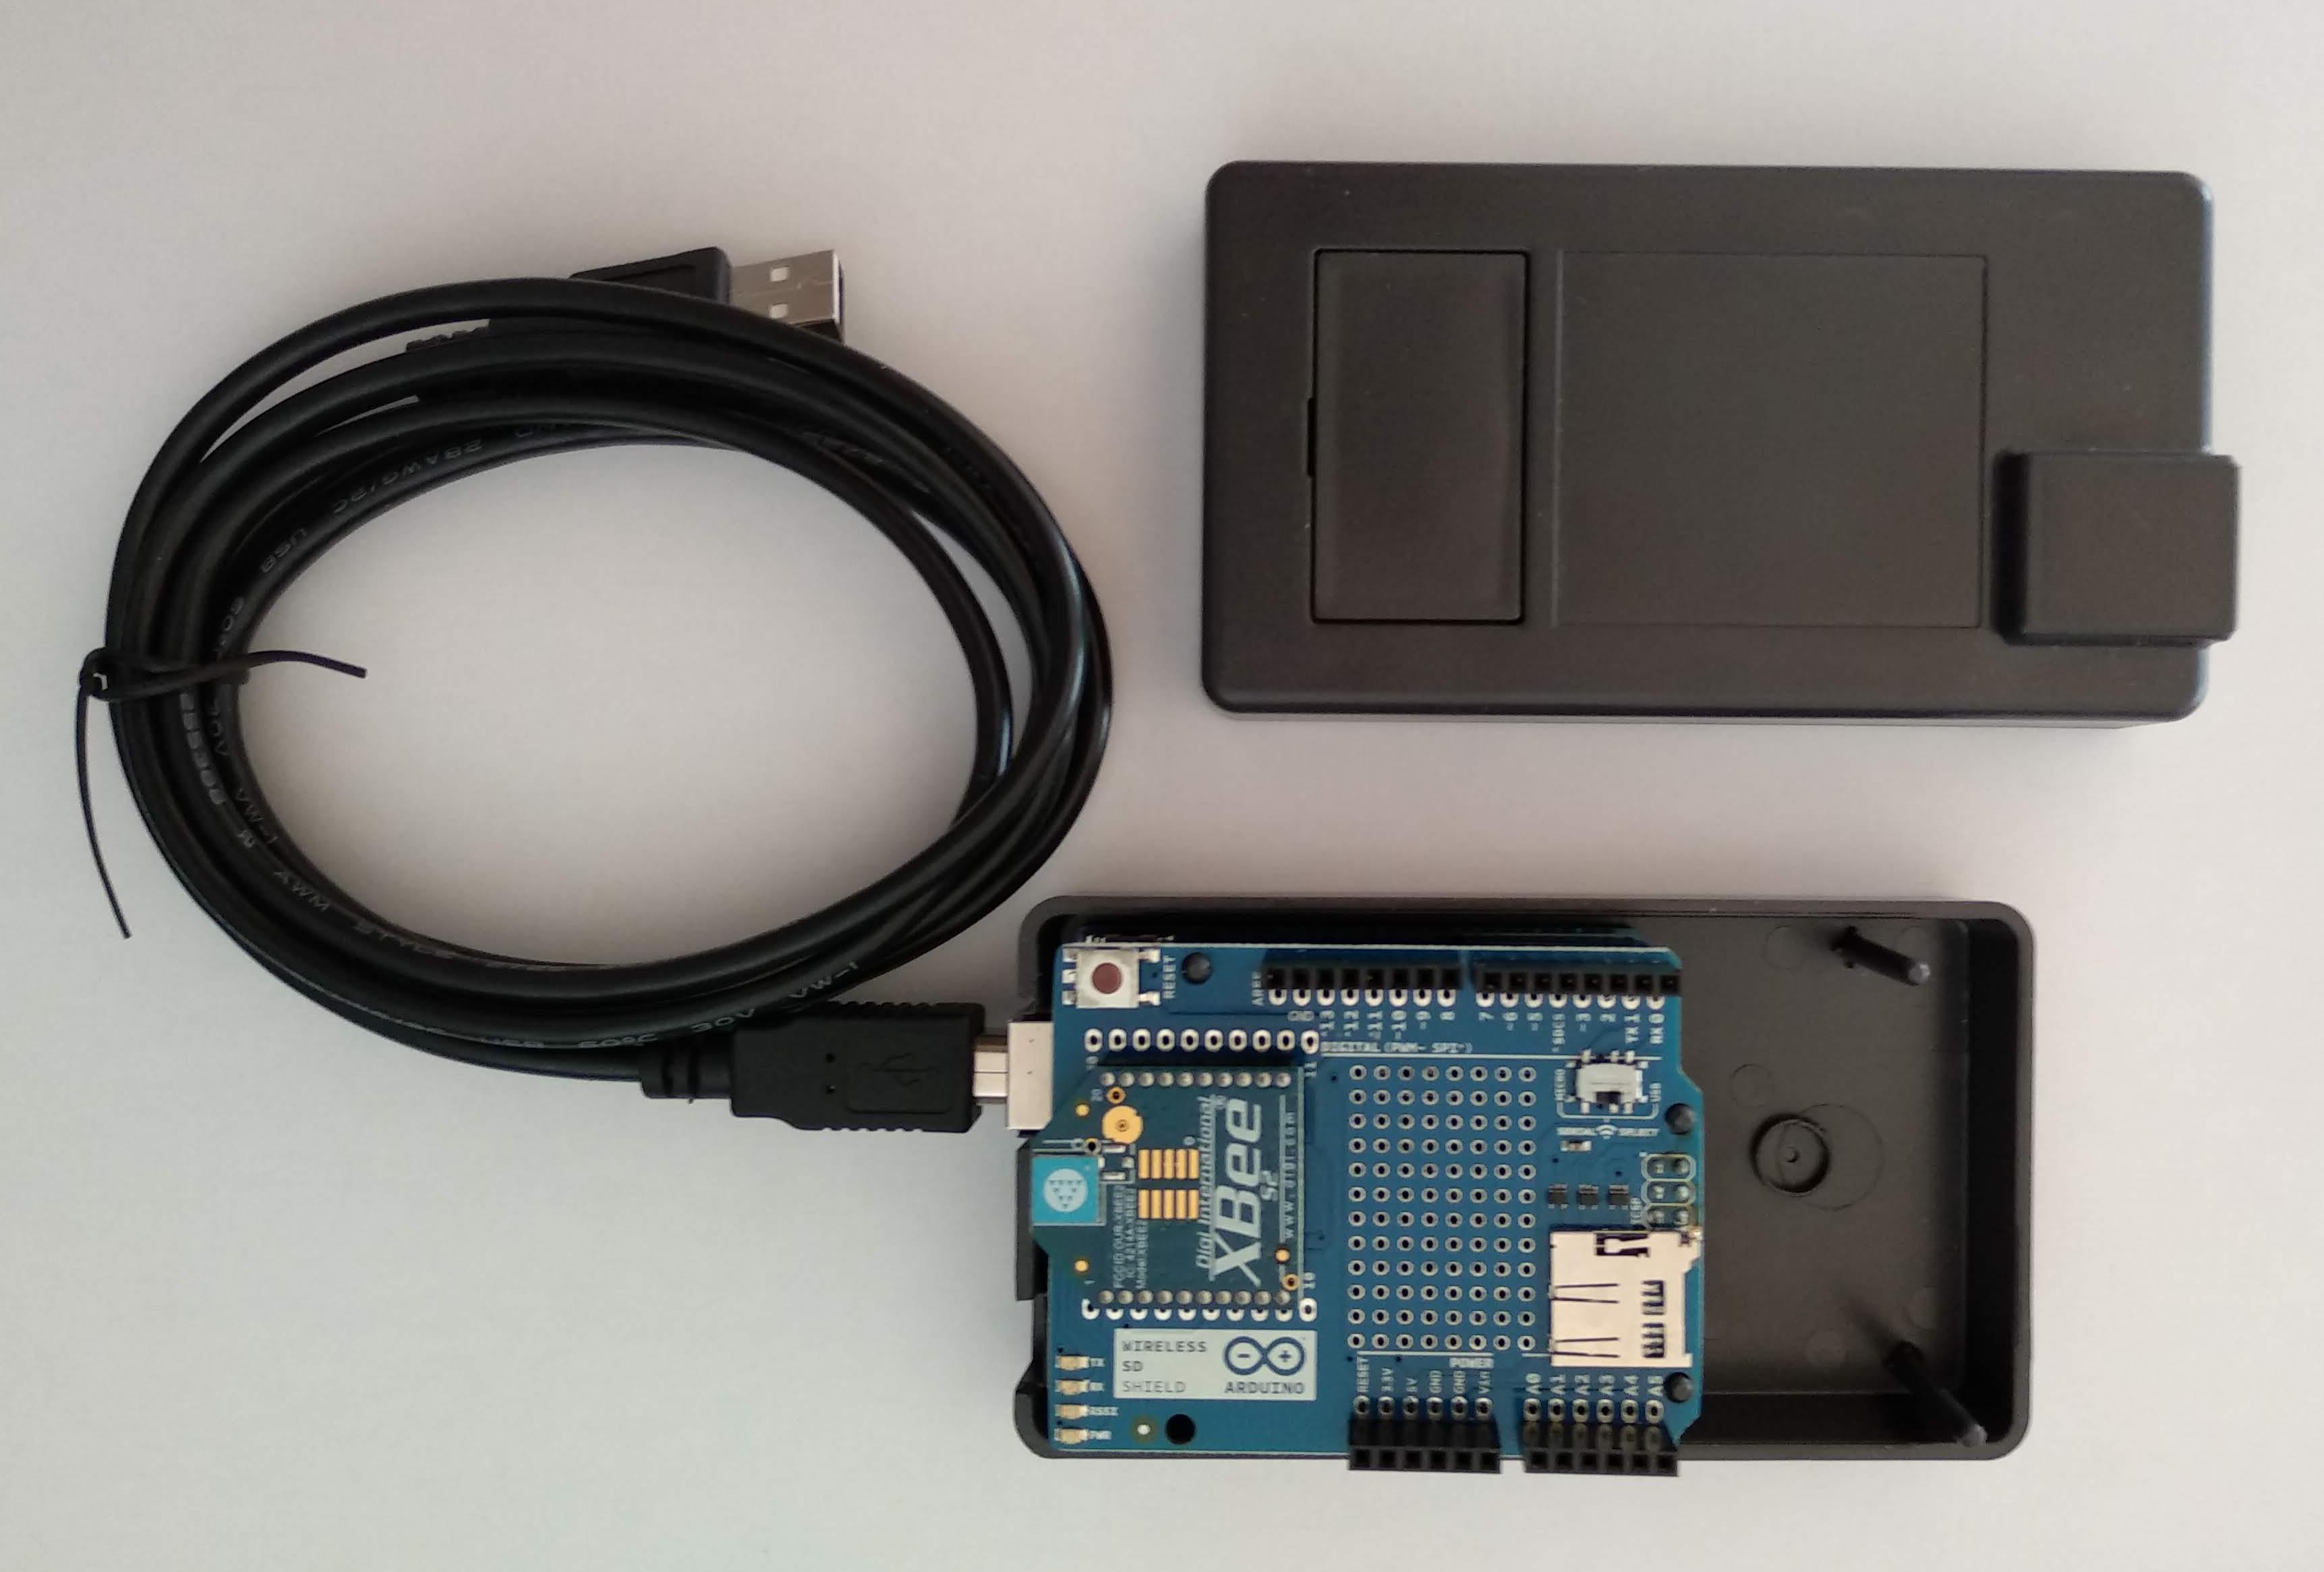
\includegraphics[scale=0.15,keepaspectratio=true]{./imagenes/router.jpg}
    % router.jpg: 640x480 pixel, 72dpi, 22.58x16.93 cm, bb=0 0 640 480
    \caption{Router}
    \label{figura:Router}
   \end{figure}
   
   A seguinte montaxe foi a do receptor, moi similar á do router, pois non deixa
   de ser unha placa Arduino Fio, que xa dispón dun zócalo para o módulo XBee e
   polo que non precisa de placa auxiliar. \\
   
   Polo mesmo motivo que o anterior, deixouse para máis adiante coma o último
   punto ou nivel de integración, pois resulta máis robusto probar e medir
   primeiro de maneira cableada e logo escalar ó modo sen fíos e poder comparar
   medicións e resultados. \\
  
   \begin{figure}[htbp]
    \centering
    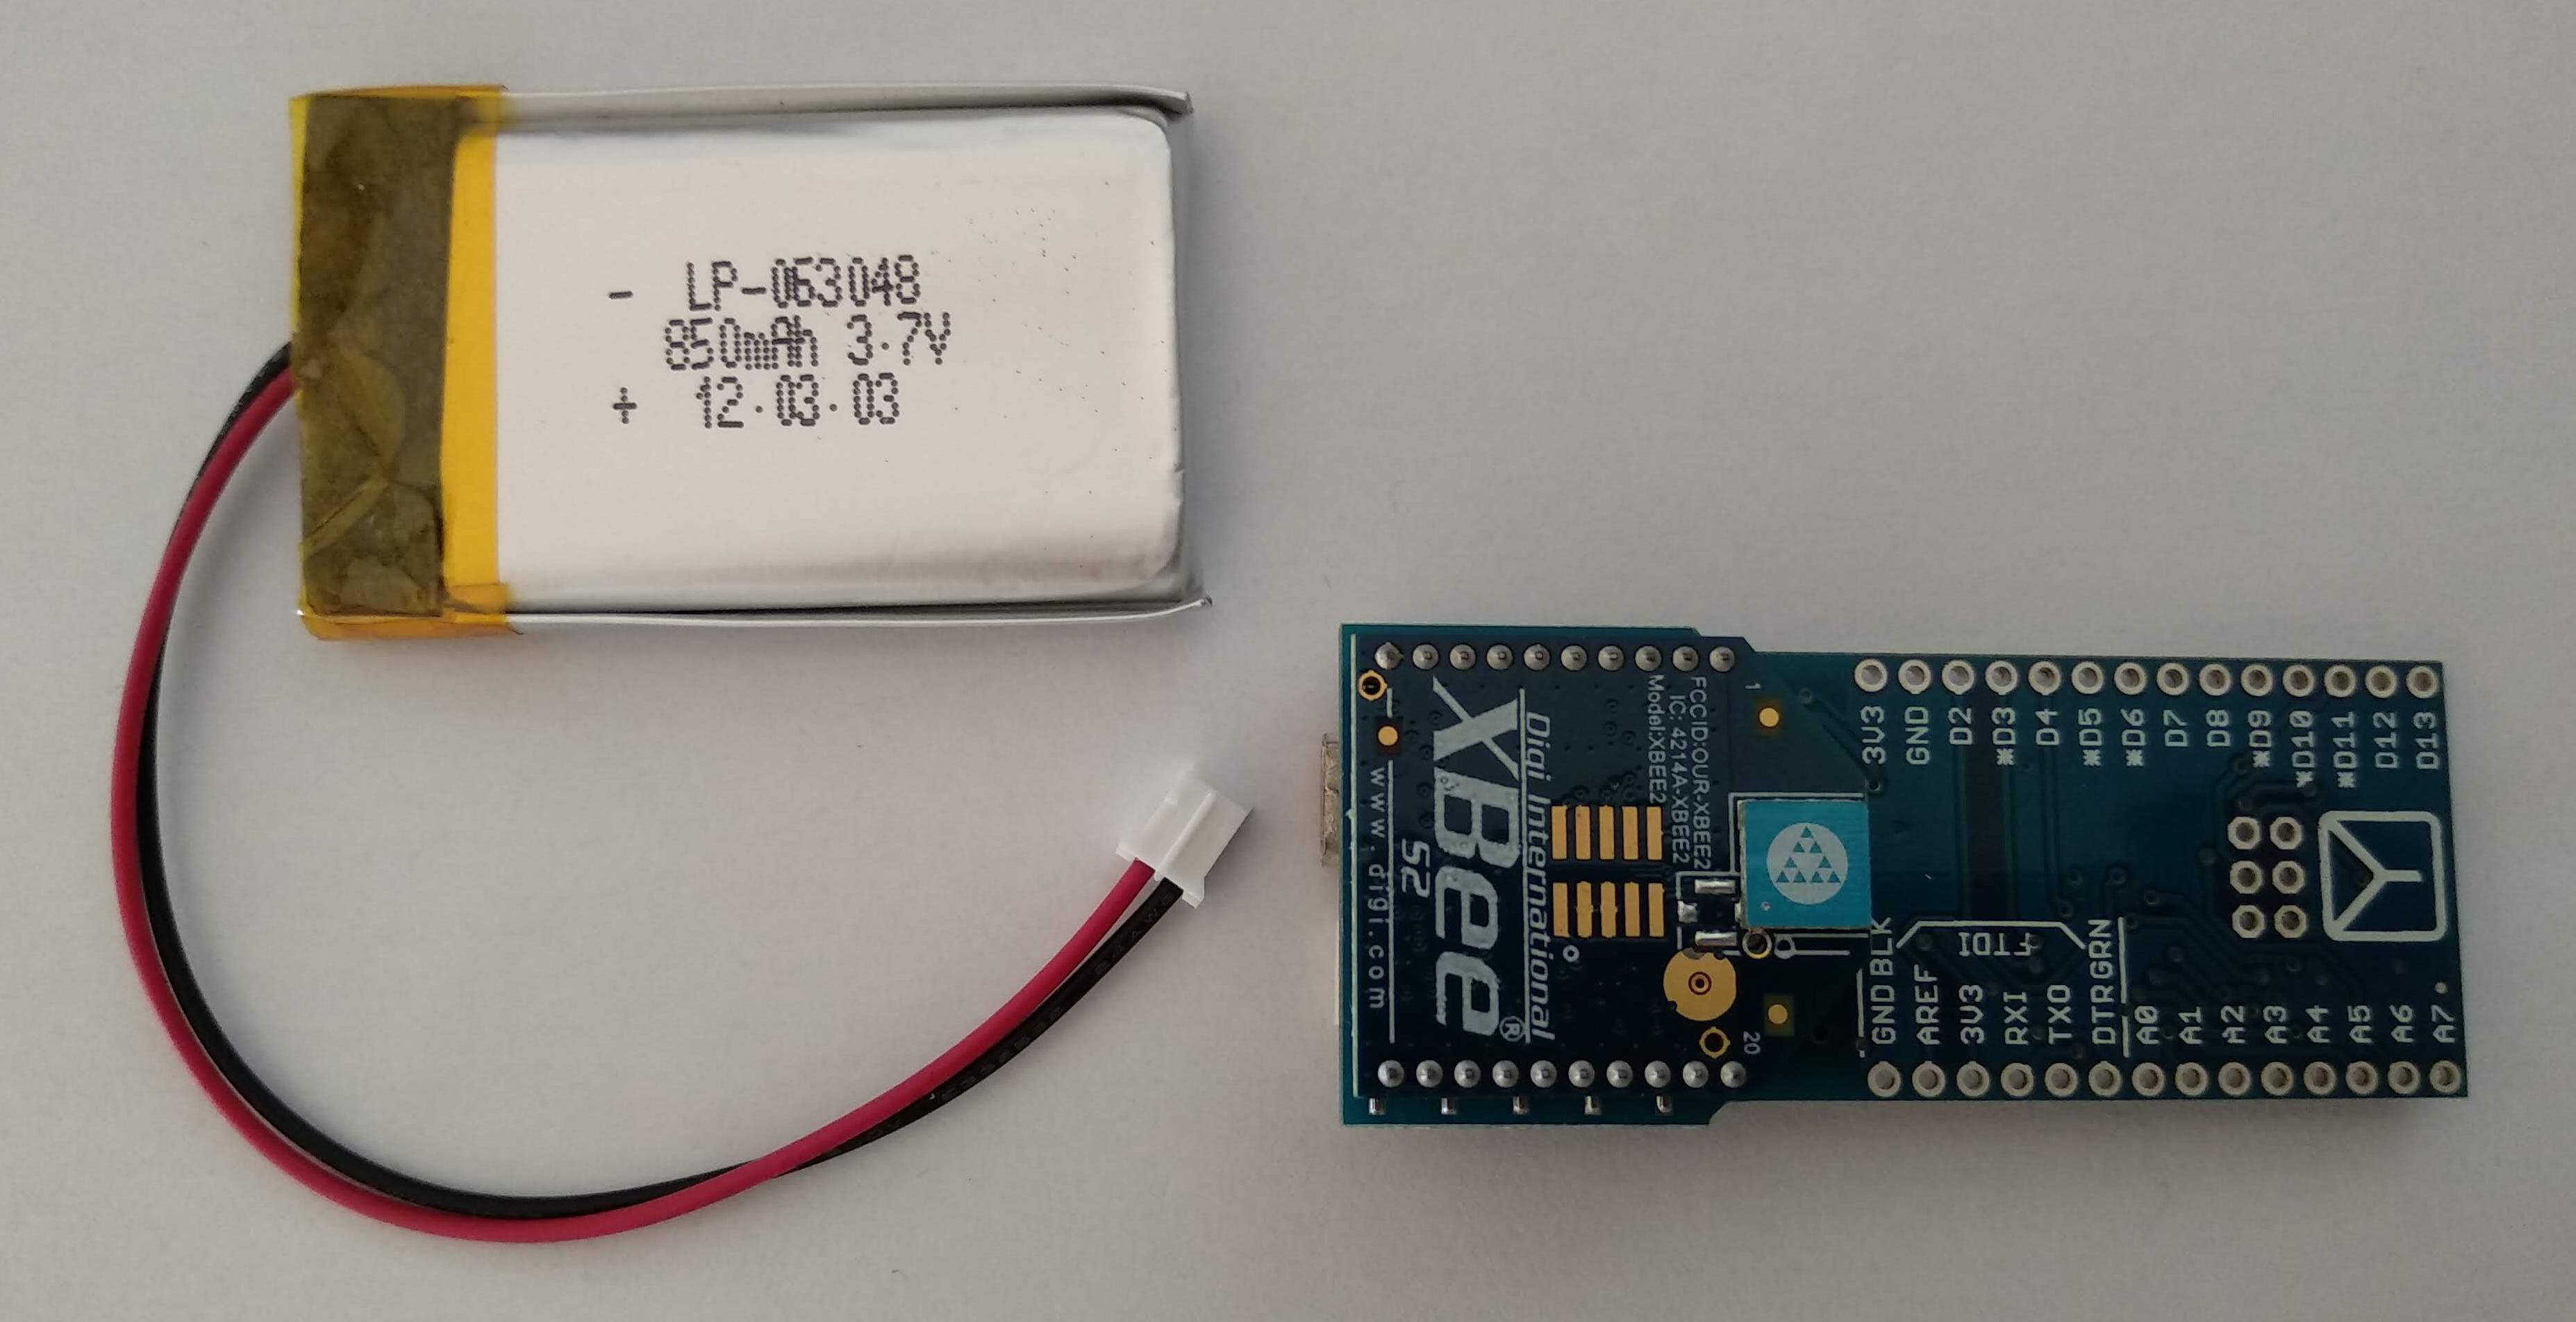
\includegraphics[scale=0.15,keepaspectratio=true]{./imagenes/receptor.jpg}
    % receptor.jpg: 640x480 pixel, 72dpi, 22.58x16.93 cm, bb=0 0 640 480
    \caption{Receptor}
    \label{figura:Receptor}
   \end{figure}
   
   No seu lugar, para desenvolver a lóxica de negocio da gaita MIDI, empregouse
   unha placa Arduino Uno, que conta coas mesmas características, salvo pola
   conexión directa do módulo XBee e que conta coa vantaxe de que podemos
   descargar nela o firmware da nosa implementación directamente a través dun
   cable USB. \\
   
   Neste caso a interface pública veu definida polo propio funcionamento de
   Arduino, contando cun método de configuración inicial e outro de execución
   continua. \\
   
   O que fixemos neste caso foi facer unha primeira implementación en
   pseudo-código do comportamento xeral que tería o dispositivo, intentando
   ver a qué periférico tería que chamar en cada caso, cándo e cómo, dando como
   resultado dúas partes claramente diferenciadas:
   
   \begin{itemize}
    \item Configuración das características propias da gaita.
    \item E reproducción ou envío de mensaxes MIDI.
   \end{itemize}
   
   Na parte de configuración, realizaríase tanto a carga dos parámetros
   configurables ó inicio coma o intercambio de configuracións entre o
   dispositivo e a aplicación de configuración, para o que sería preciso tirar
   do lector de tarxetas para persistir a información, así coma unha librería
   JSON para darlle formato un formato usable á mesma e da que falaremos máis
   adiante. \\
   
   En canto á parte de reproducción, sería preciso avaliar a presión do fol para
   decidir se o dispositivo debe soar ou non e a dixitación actual a través dos
   sensores capacitivos para ver se corresponde con algunha válida e por tanto
   producir o son relativo á mesma mediante o emprego dunha librería MIDI da que
   tamén falaremos máis adiante. \\
   
   Ampliaremos esta lóxica polo miúdo cando cheguemos á parte software, facendo
   uso de diagramas de fluxo. \\
   
   A continuación procedeuse co sensor de presión, por ser o seguinte máis
   sinxelo en orde de funcionalidade, pois o único que precisamos obter del é a
   presión dentro do fol, aínda que pode devolver máis parámetros relacionados
   coa mesma. \\
   
   Como se pode ver na imaxe, conectouse a unha placa Arduino Uno empregando
   o bus I2C do mesmo. \\
  
   \begin{figure}[htbp]
    \centering
    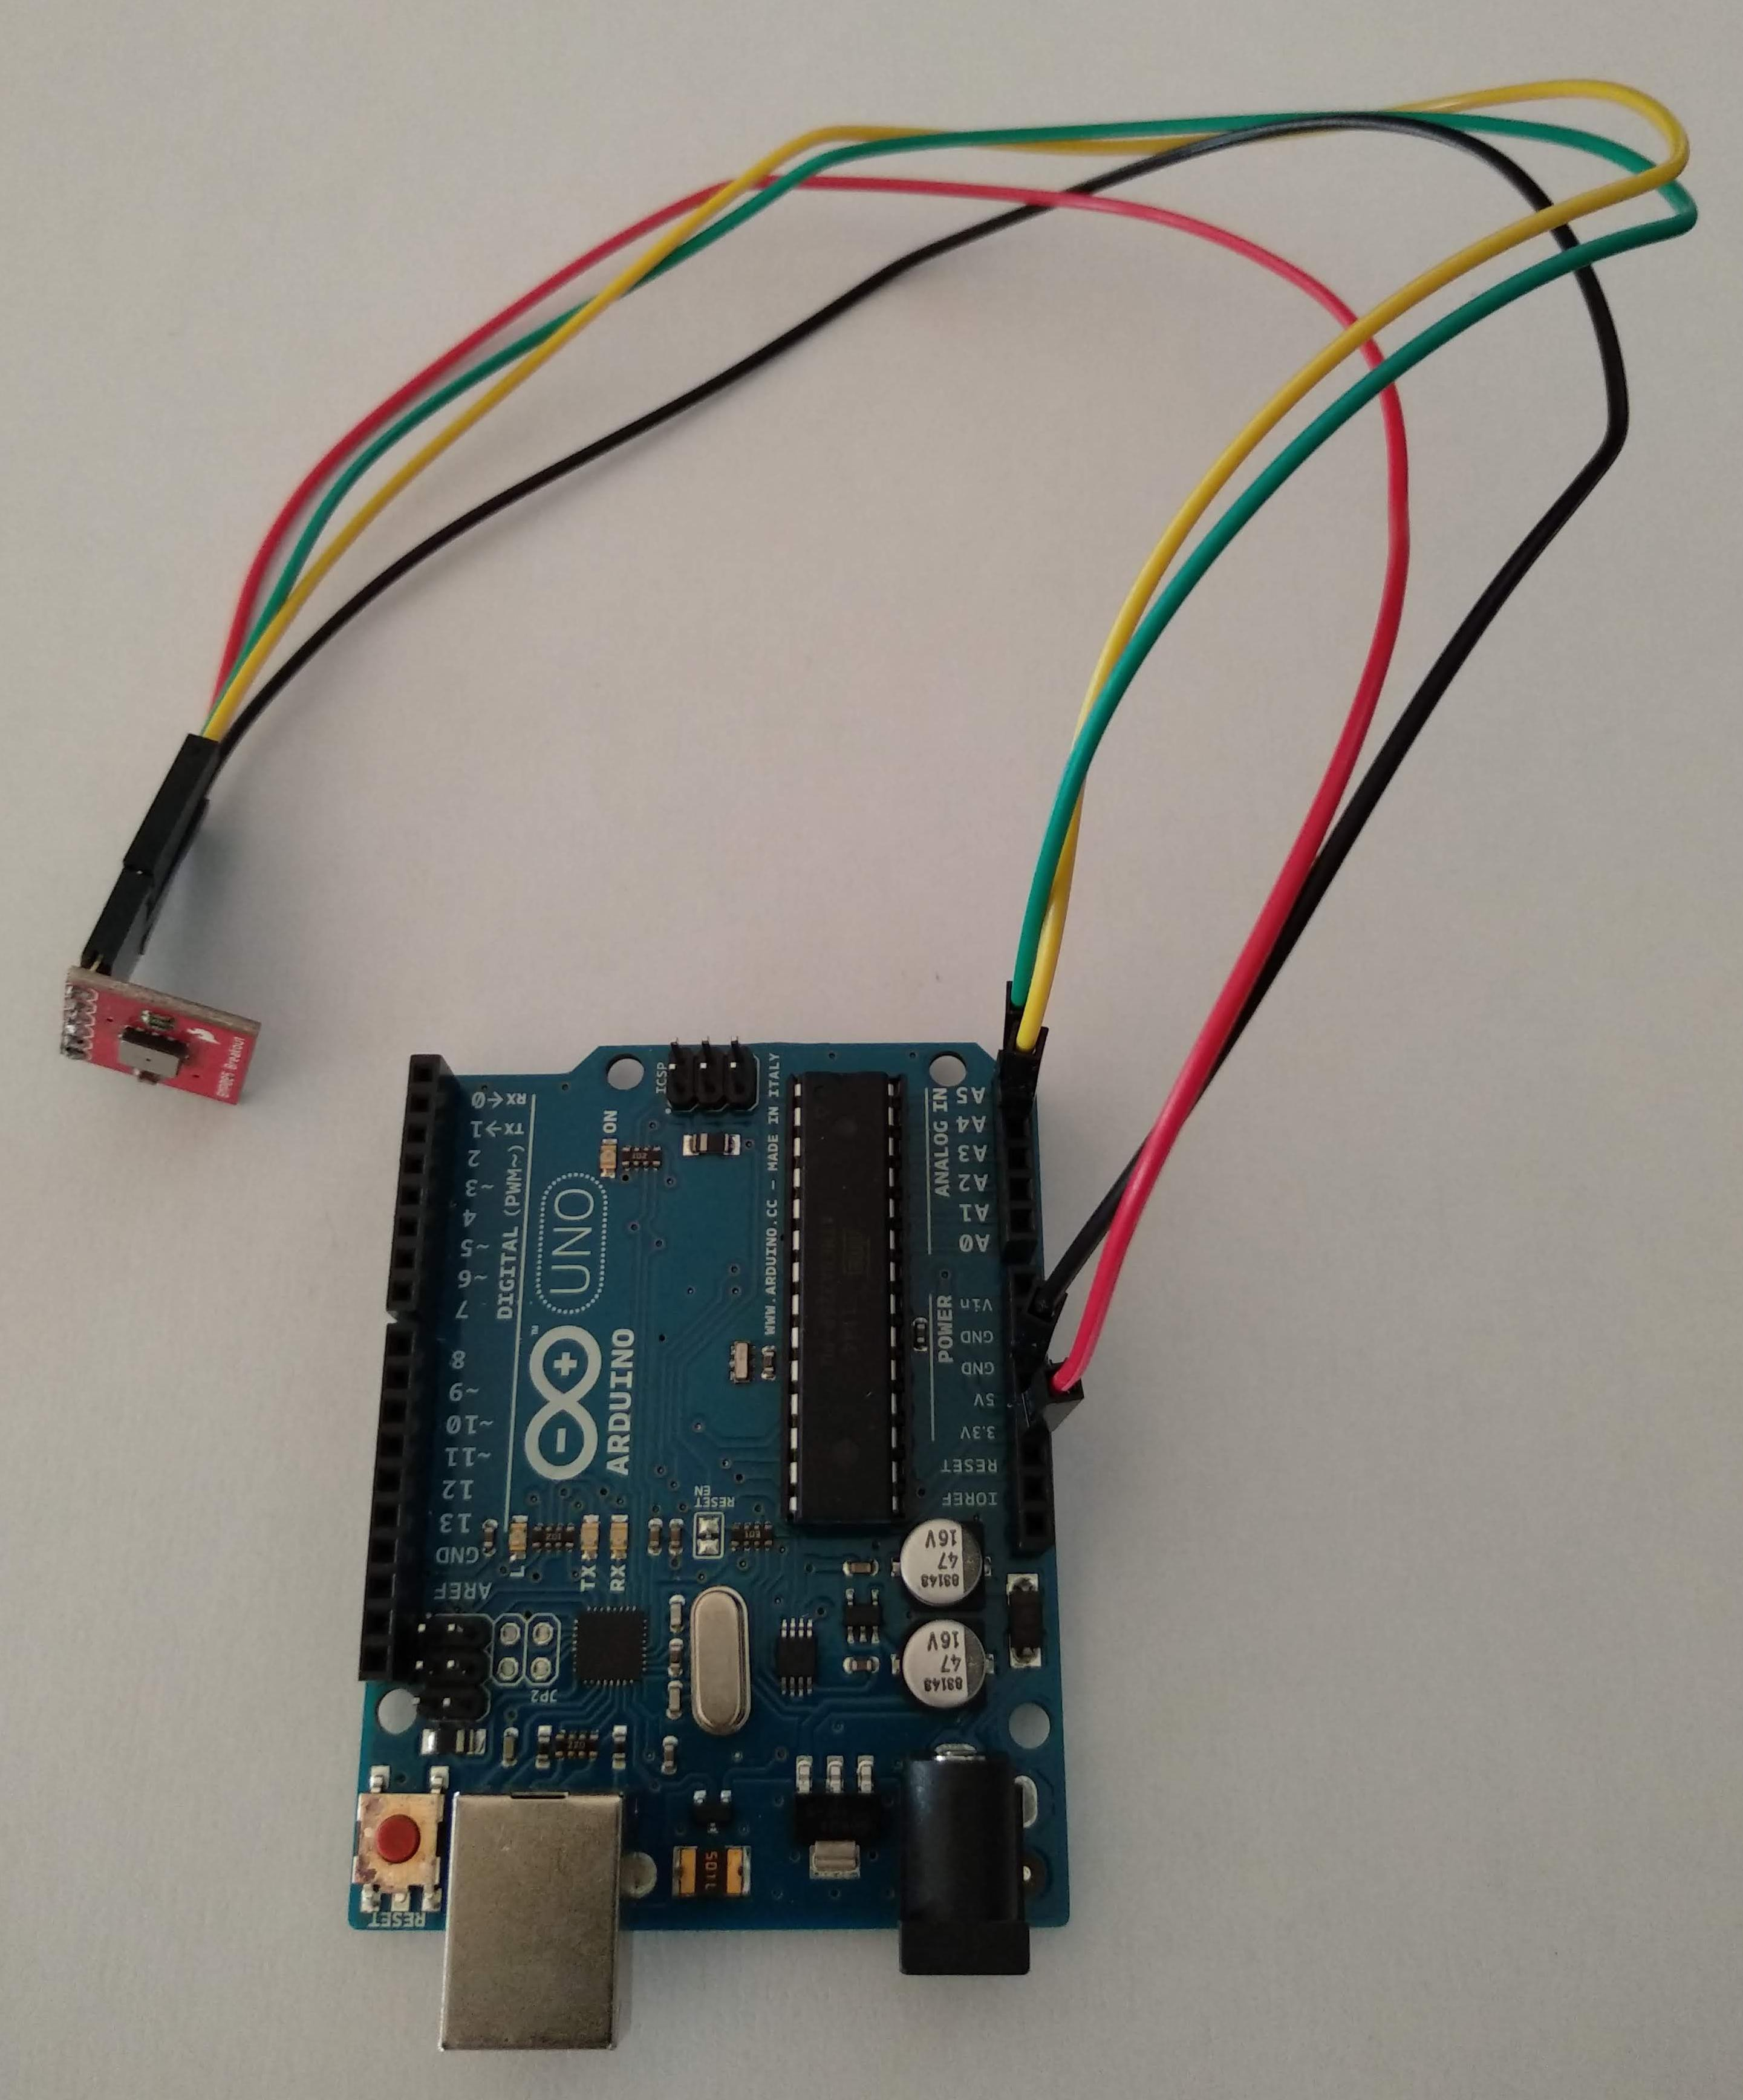
\includegraphics[scale=0.2,keepaspectratio=true]{./imagenes/sensor-presion.jpg}
    % sensor-presion.jpg: 640x480 pixel, 72dpi, 22.58x16.93 cm, bb=0 0 640 480
    \caption{Sensor de presión}
    \label{figura:SensorPresion}
   \end{figure}
   
   Ademáis de definir a súa interface pública (figura 
   \ref{figura:InterfaceSensorPresion}) para a obtención da presión e un
   ficheiro de proba (figura \ref{figura:TestSensorPresion}) para validar a
   implementación completa posterior. \\
   
   \begin{figure}[htbp]
    \centering
    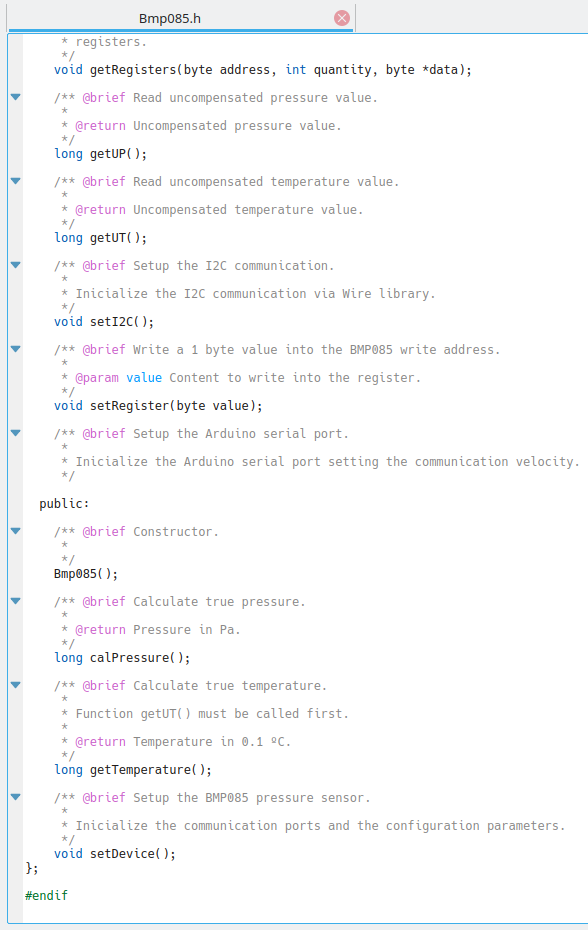
\includegraphics[scale=0.8,keepaspectratio=true]{./imagenes/interface-sensor-presion.png}
    % interface-sensor-presion.png: 640x480 pixel, 72dpi, 22.58x16.93 cm, bb=0 0 640 480
    \caption{Interface do sensor de presión}
    \label{figura:InterfaceSensorPresion}
   \end{figure}
   
   \begin{figure}[htbp]
    \centering
    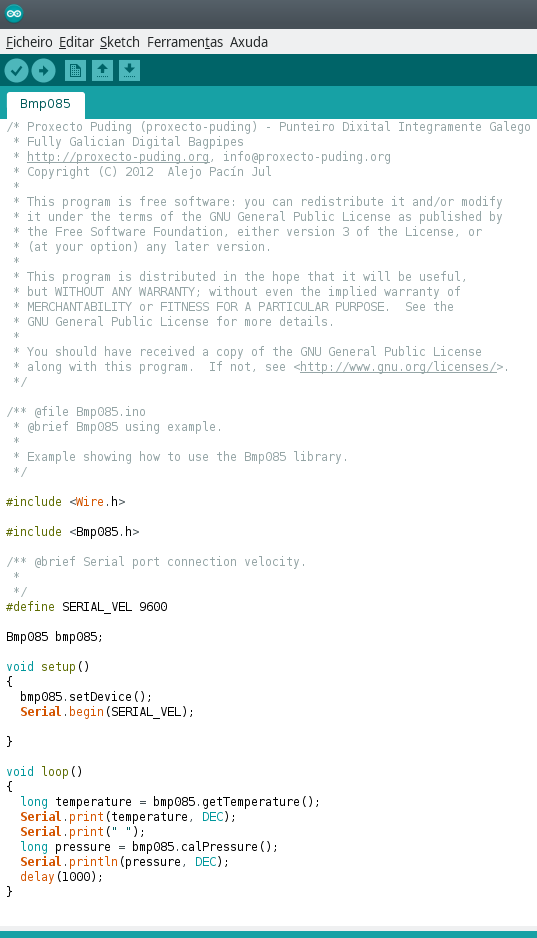
\includegraphics[scale=0.8,keepaspectratio=true]{./imagenes/test-sensor-presion.png}
    % test-sensor-presion.png: 640x480 pixel, 72dpi, 22.58x16.93 cm, bb=0 0 640 480
    \caption{Ficheiro de proba do sensor de presión}
    \label{figura:TestSensorPresion}
   \end{figure}
   
   O turno seguinte foi para os sensores capacitivos. Neste caso, o que
   precisamos saber é cáles están acesos en cada momento, de maneira que
   poidamos facer \textit{pattern matching} contra a configuración da gaita e
   saber se teriamos algún son asociado a dita dixitación, para posteriormente
   reproducilo. \\
   
   Como se pode ver na imaxe, conectouse a unha placa Arduino Uno empregando
   o bus I2C do mesmo. \\
  
   \begin{figure}[htbp]
    \centering
    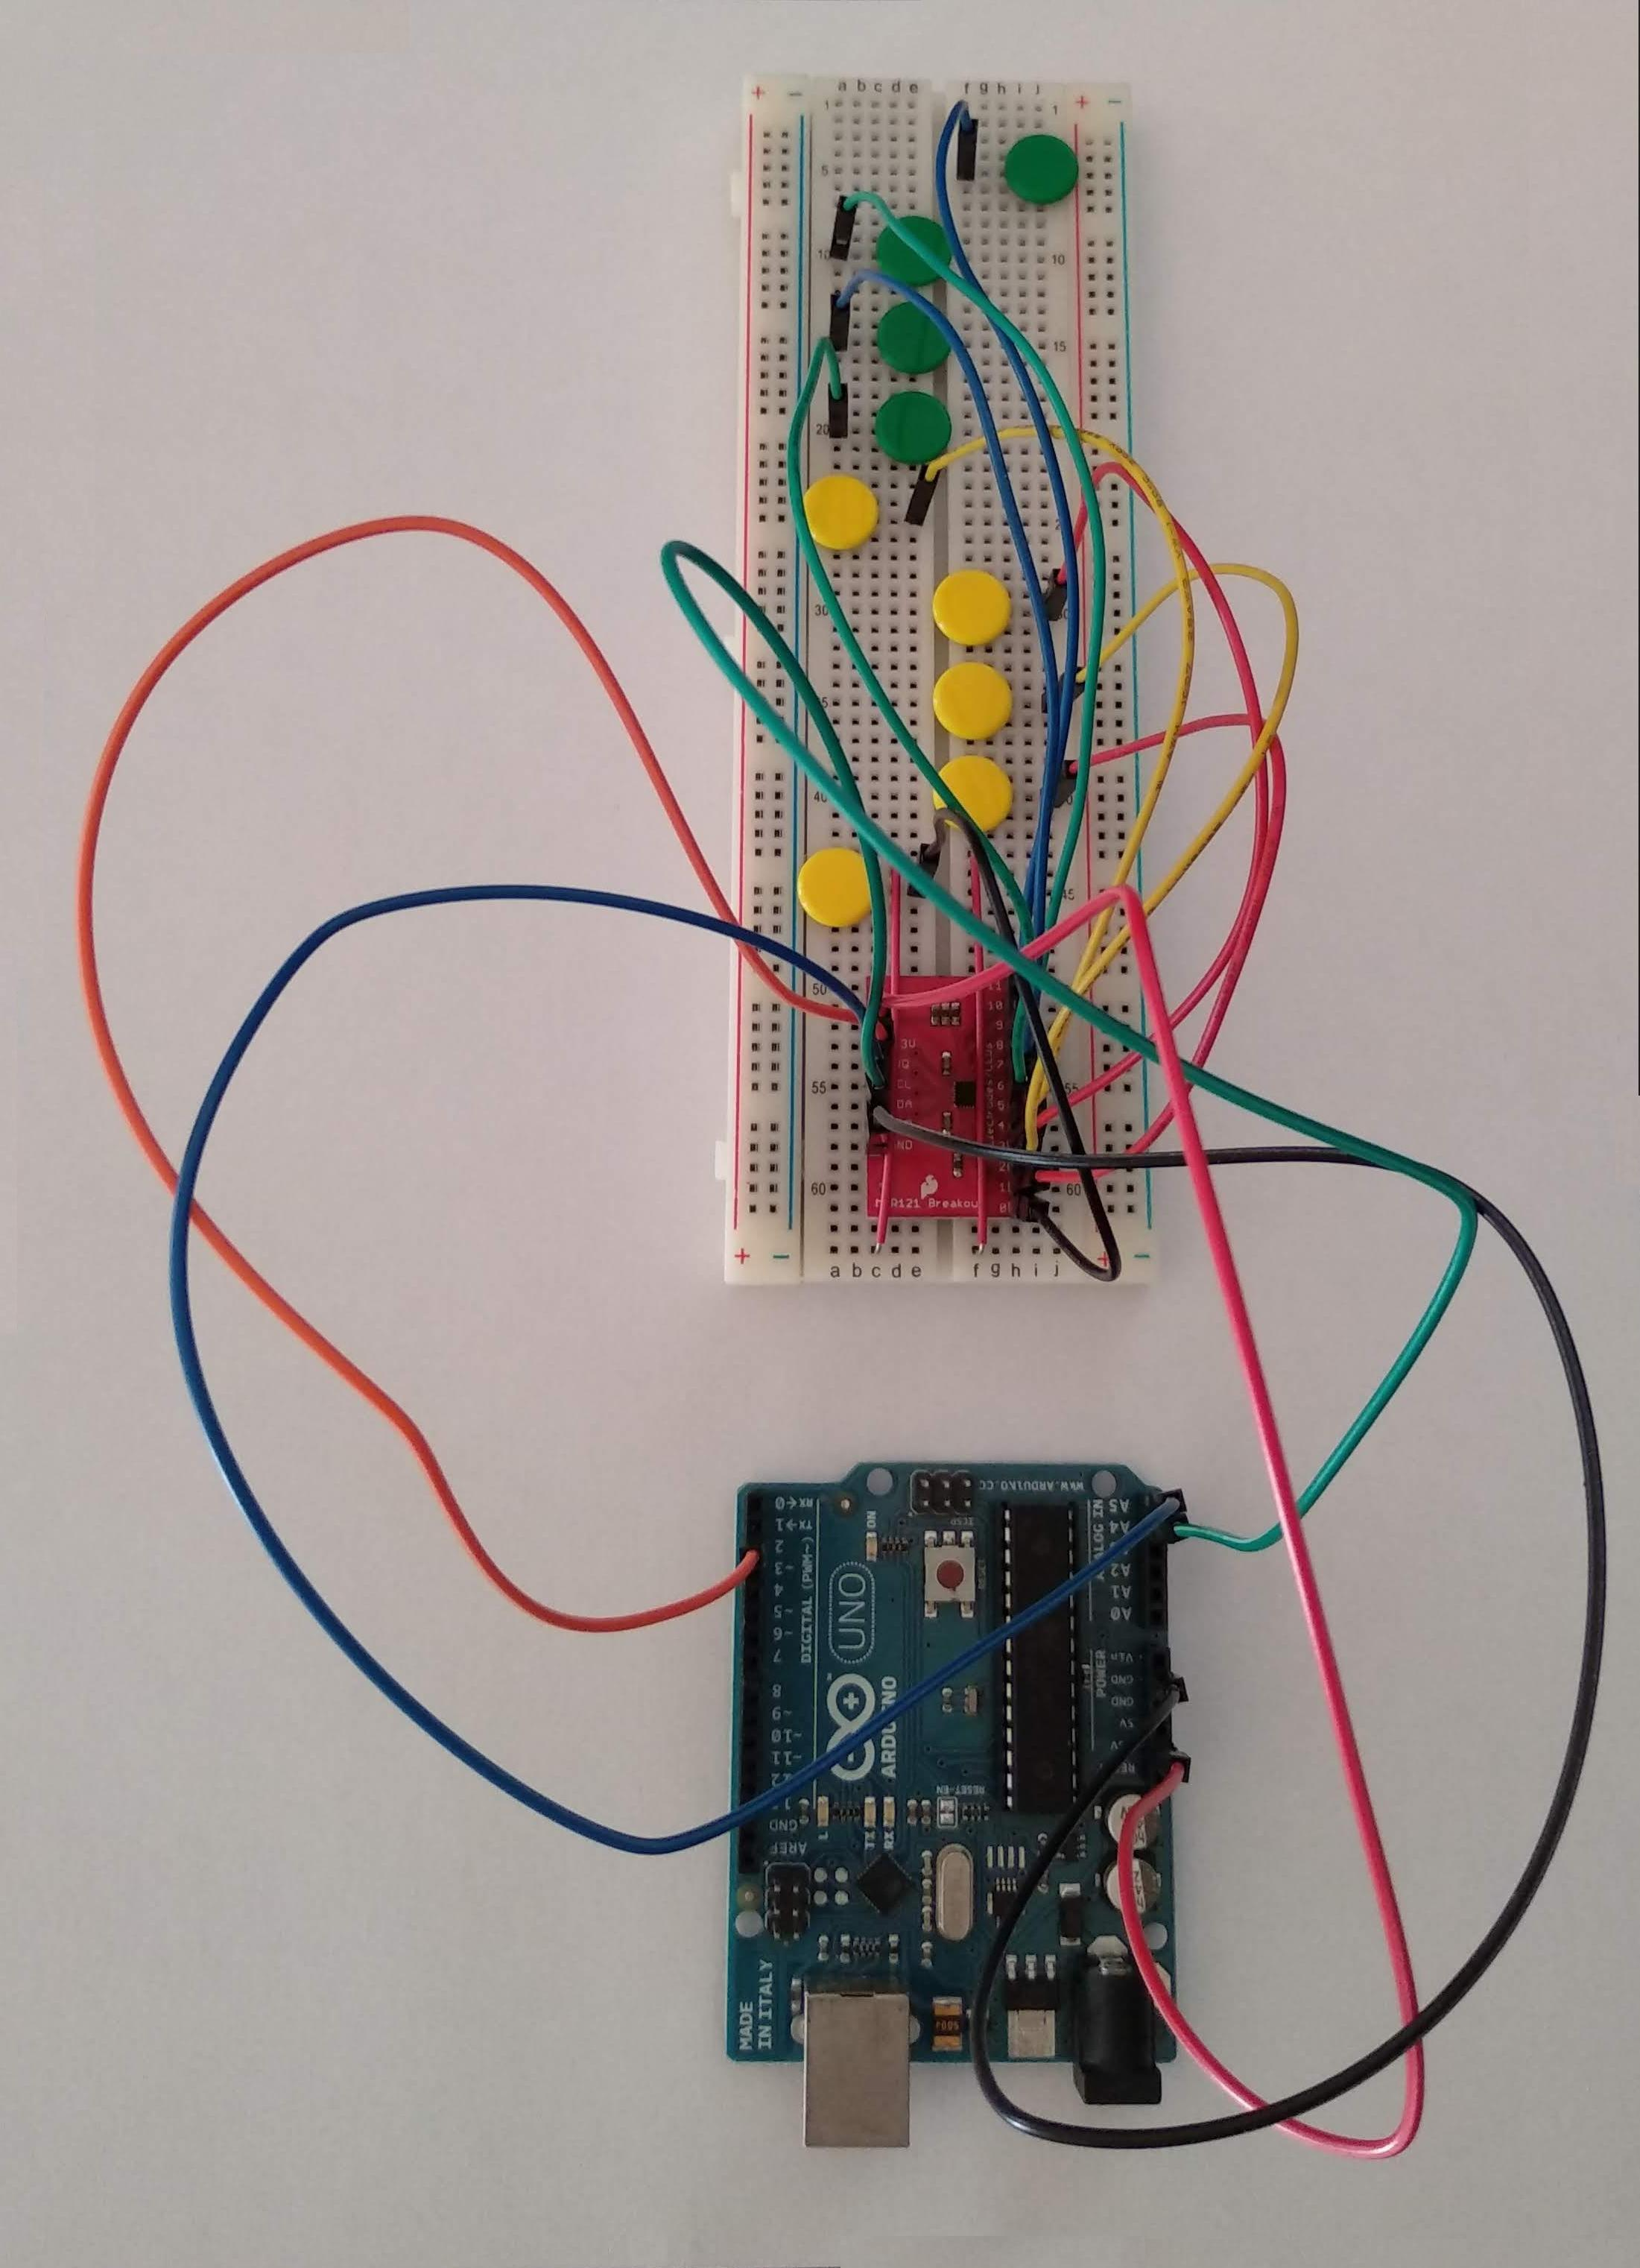
\includegraphics[scale=0.2,keepaspectratio=true]{./imagenes/sensores-capacitivos.jpg}
    % sensores-capacitivos.jpg: 640x480 pixel, 72dpi, 22.58x16.93 cm, bb=0 0 640 480
    \caption{Sensores capacitivos}
    \label{figura:SensoresCapacitivos}
   \end{figure}
   
   Ademáis de definir a súa interface pública (figura 
   \ref{figura:InterfaceSensoresCapacitivos}) para a obtención da dixitación e
   un ficheiro de proba (figura \ref{figura:TestSensoresCapacitivos}) para
   validar a implementación completa posterior. \\
   
   \begin{figure}[htbp]
    \centering
    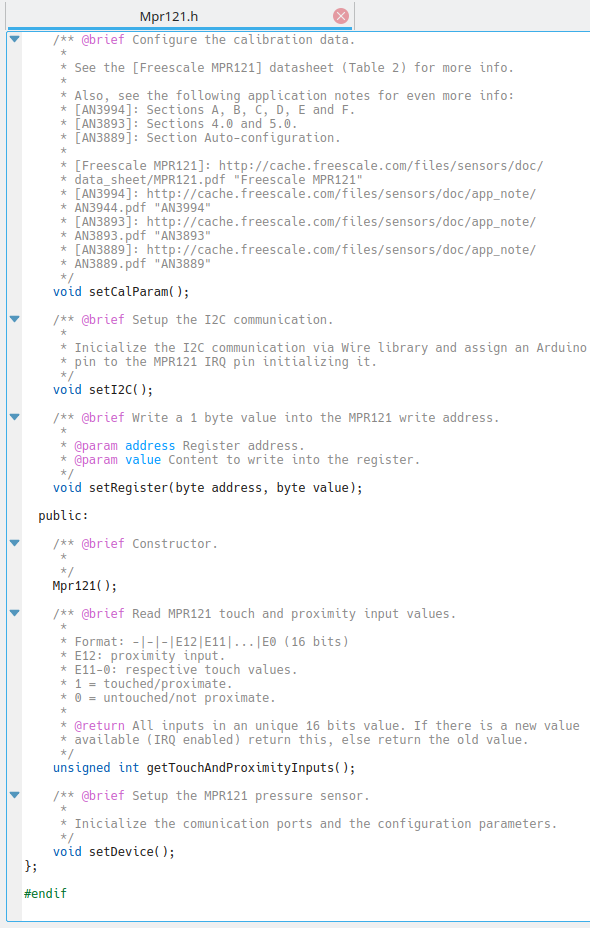
\includegraphics[scale=0.8,keepaspectratio=true]{./imagenes/interface-sensores-capacitivos.png}
    % interface-sensores-capacitivos.png: 640x480 pixel, 72dpi, 22.58x16.93 cm, bb=0 0 640 480
    \caption{Interface dos sensores capacitivos}
    \label{figura:InterfaceSensoresCapacitivos}
   \end{figure}
   
   \begin{figure}[htbp]
    \centering
    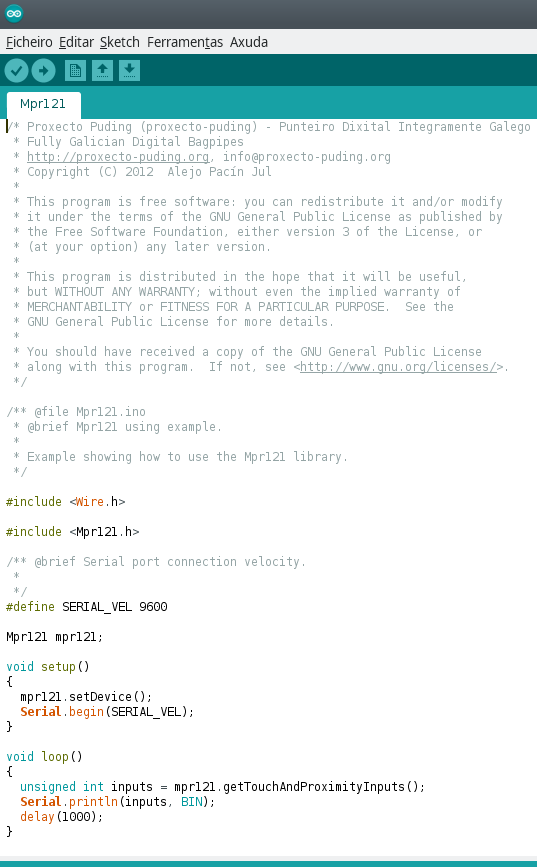
\includegraphics[scale=0.8,keepaspectratio=true]{./imagenes/test-sensores-capacitivos.png}
    % test-sensores-capacitivos.png: 640x480 pixel, 72dpi, 22.58x16.93 cm, bb=0 0 640 480
    \caption{Ficheiro de proba dos sensores capacitivos}
    \label{figura:TestSensoresCapacitivos}
   \end{figure}
   
   Para rematar cos periféricos, procedeuse co lector de tarxetas. Neste caso o
   que precisamos é poder ler e almacenar a configuración variable do
   dispositivo, de maneira que sexa independente e única para cada un dos
   mesmos. \\
   
   Como se pode ver na imaxe, conectouse a unha placa Arduino Uno empregando
   o porto UART do mesmo. \\
  
   \begin{figure}[htbp]
    \centering
    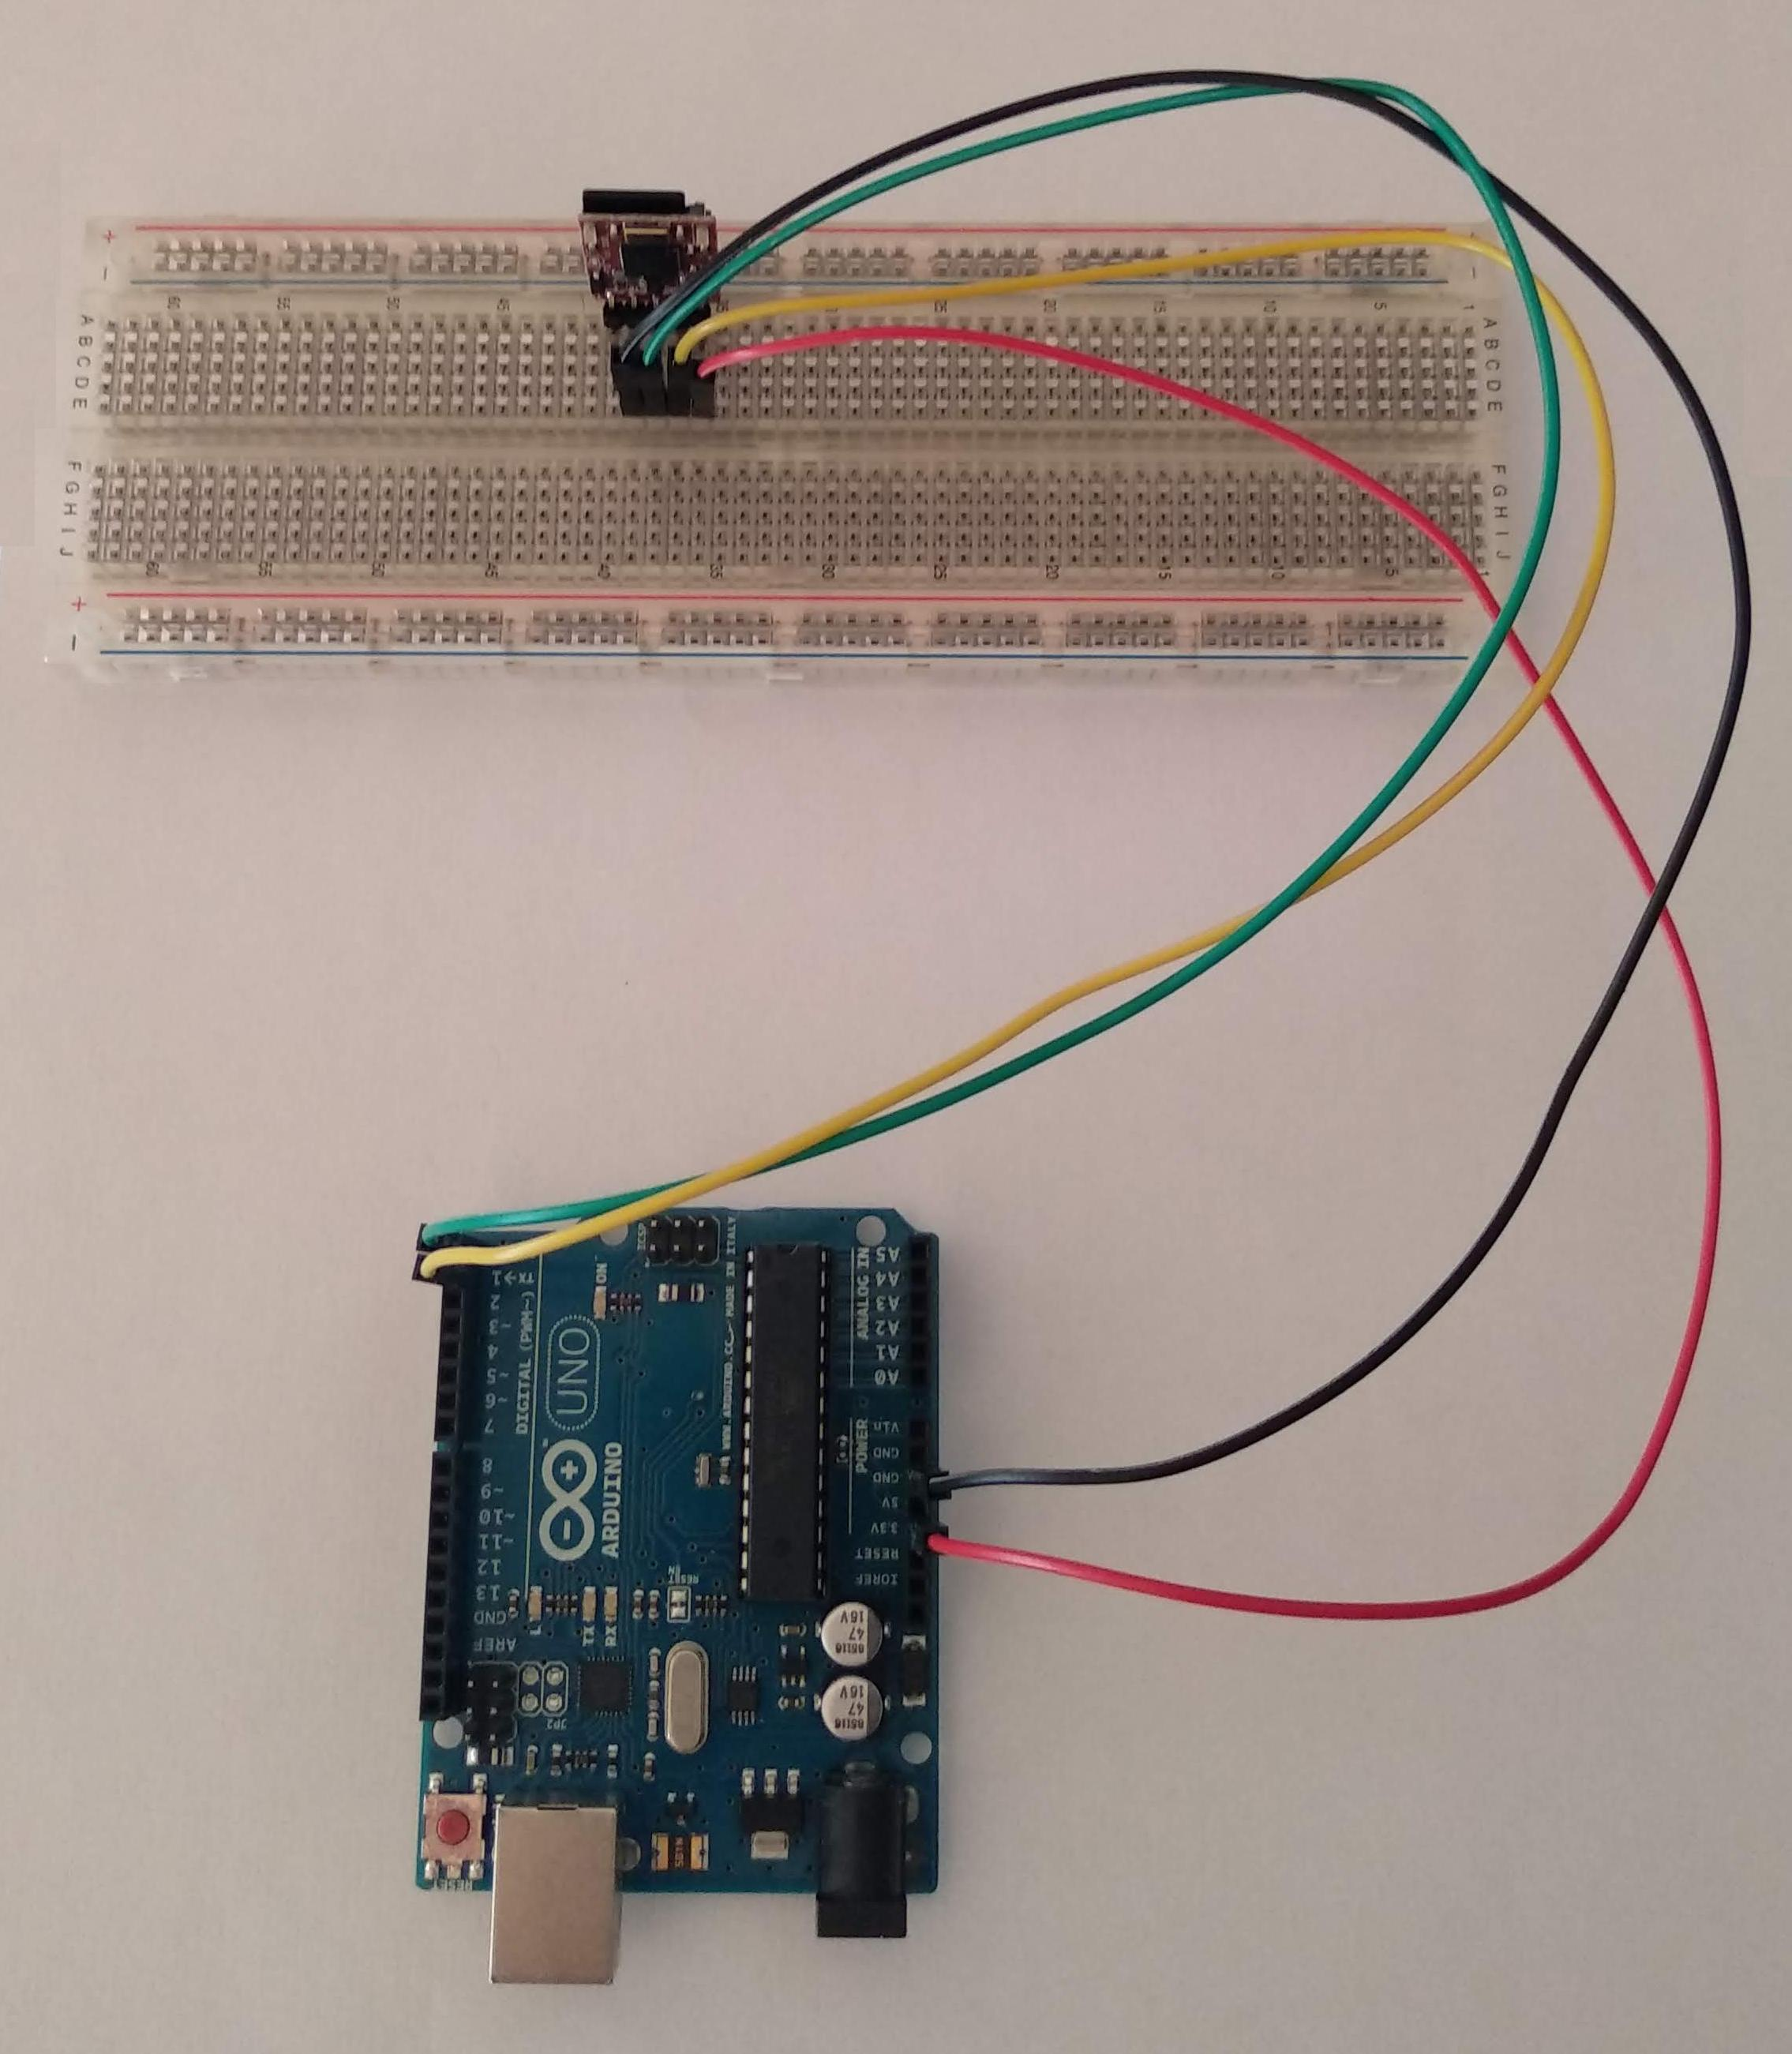
\includegraphics[scale=0.2,keepaspectratio=true]{./imagenes/lector-tarxetas.jpg}
    % lector-tarxetas.jpg: 640x480 pixel, 72dpi, 22.58x16.93 cm, bb=0 0 640 480
    \caption{Lector de tarxetas}
    \label{figura:LectorTarxetas}
   \end{figure}
   
   Ademáis de definir a súa interface pública (figura 
   \ref{figura:InterfaceLectorTarxetas}) para a obtención da configuración e un
   ficheiro de proba (figura \ref{figura:TestLectorTarxetas}) para validar a
   implementación completa posterior. \\
   
   \begin{figure}[htbp]
    \centering
    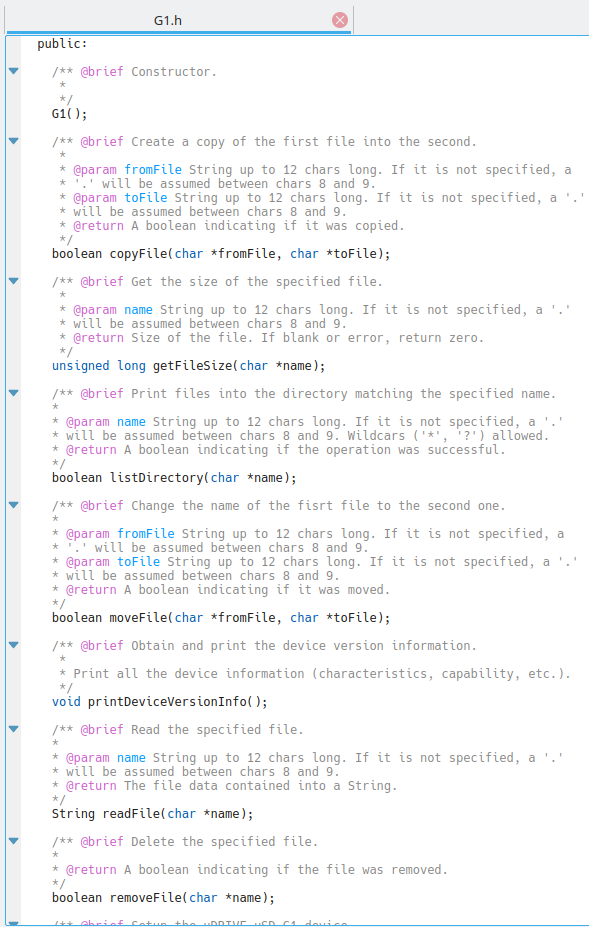
\includegraphics[scale=0.8,keepaspectratio=true]{./imagenes/interface-lector-tarxetas.png}
    % interface-lector-tarxetas.png: 640x480 pixel, 72dpi, 22.58x16.93 cm, bb=0 0 640 480
    \caption{Interface do lector de tarxetas}
    \label{figura:InterfaceLectorTarxetas}
   \end{figure}
   
   \begin{figure}[htbp]
    \centering
    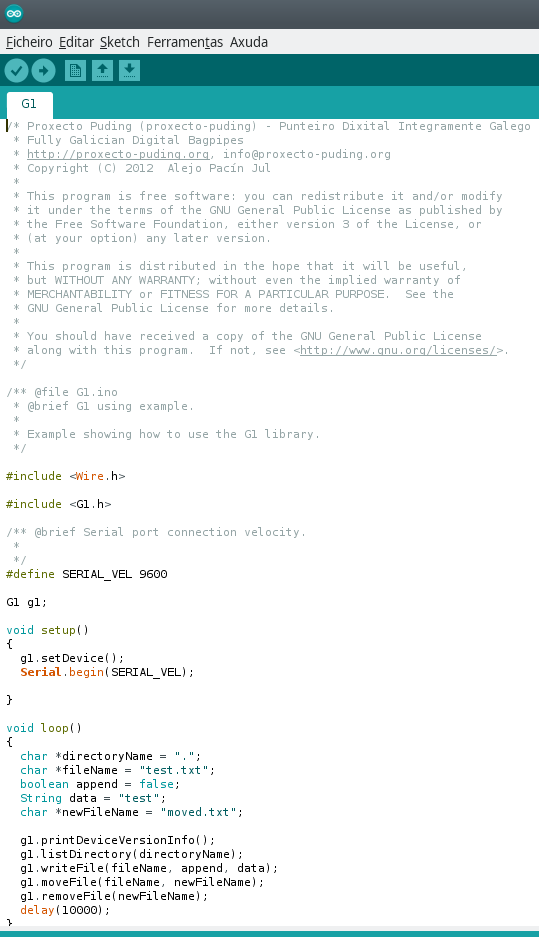
\includegraphics[scale=0.8,keepaspectratio=true]{./imagenes/test-lector-tarxetas.png}
    % test-lector-tarxetas.png: 640x480 pixel, 72dpi, 22.58x16.93 cm, bb=0 0 640 480
    \caption{Ficheiro de proba do lector de tarxetas}
    \label{figura:TestLectorTarxetas}
   \end{figure}

   \paragraph{Encapsulamento do hardware}
   
   Debido a atoparse nunha situación temperá do prototipado físico, o
   encapsulamento do hardware realizouse da maneira máis leve posible, dada a
   necesidade de poder montar e desmontar a vontade durante as probas. \\
   
   Como pode comprobarse nas imaxes do apartado anterior, o único elemento
   encapsulado por completo sería o router e o resto estaría ó aire, facendo uso
   de cables de prototipado para evitar ter que soldar e desoldar durante as
   probas. \\
   
   Ademáis, cada un dos periféricos foi montado por separado ata a integración
   completa do hardware, logo da correcta implementación, verificación e
   validación do mesmo.

  \subsubsection{Prototipo software}
  
  Para a o prototipo software operacional tiramos do prototipo deseñado na fase
  anterior e dos diagramas UML relacionados.

   \paragraph{Desenvolvemento do prototipo}

   \paragraph{Gravación das mostras}

\section{Desenvolvemento e validación do seguinte nivel do producto}

 \subsection{Simulacións, modelos e programas de proba}

 \subsection{Deseño detallado}

  \subsubsection{Deseño hardware}

  \subsubsection{Deseño software}

 \subsection{Ensamblado e codificación}

  \subsubsection{Ensamblado}

  \subsubsection{Codificación}

 \subsection{Probas de unidade}

 \subsection{Integración e probas}

 \subsection{Probas de aceptación}

 \subsection{Implantación}
